\chapter{Метод обучения с подкреплением} \label{chapt1}

\section{Постановка задачи обучения с подкреплением} \label{sect1_1}
\begin{figure}[ht] 
	\center
	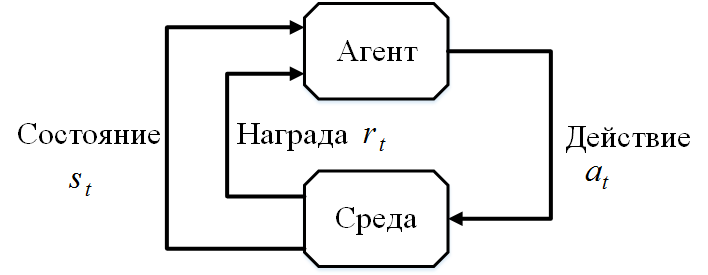
\includegraphics [scale=0.7] {rl}
	\caption{Схема взаимодействия агента со средой} 
	\label{img:rl}  
\end{figure}

%\newpage
%============================================================================================================================

\section{Функции оценки} \label{sect1_2}

\section{Алгоритмы обучения} \label{sect1_3}

\subsection{Алгоритм временных разностей} \label{subsect1_3_1}

\subsection{Алгоритм SARSA} \label{subsect1_3_2}

\subsection{Алгоритм Q-обучения} \label{subsect1_3_3}

Q-обучение это алгоритм, в основе которого лежит отложенное  вознаграждение [Уоткинс 89]. Целью данного алгоритма является максимизация Q(s, a) – ожидаемого дисконтированного вознаграждения рассчитанного для действия а при состоянии s. Алгоритм рассчитывает и обновляет значения Q для каждой комбинации «состояние-действие»

\begin{equation}
\label{eq:1_3_3p1}
\begin{alignedat}{2}
s' \leftarrow T(s,a),\\
E(s)=max_{a}Q(s,a),\\
Q(s,a)=r + \gamma(E(s')).
\end{alignedat}
\end{equation}

Q расчитывается по следующему правилу:

\begin{equation}
\label{eq:1_3_3p2}
\begin{alignedat}{2}
Q(s,a) \leftarrow Q(s,a) + \beta(r + \gamma E(s') - Q(s,a)), 0 \le \gamma \le 1.
\end{alignedat}
\end{equation}

\subsection{Алгоритм $TD(\lambda)$} \label{subsect1_3_4}

\subsection{Метод Актор-Критик} \label{subsect1_3_5}

\begin{figure}[ht] 
	\center
	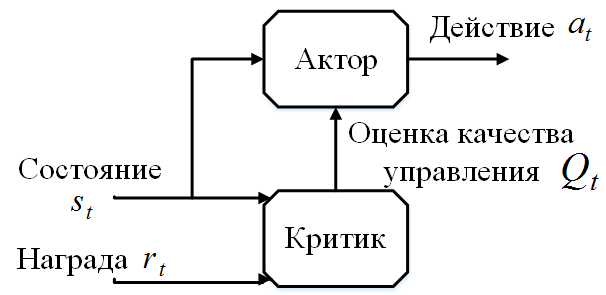
\includegraphics [scale=0.7] {ac}
	\caption{Схема взаимодействия агента со средой} 
	\label{img:ac}  
\end{figure}

\subsection{Анализ алгоритмов обучения} \label{subsect1_3_6}

